\clearpage
\section{NPC 的图片与场景查询}

物理实验台上方有一个红箱子。离线工具从 32 个标定好的机位读取场景的图像。“标定好”指我们知道相机放在哪里、朝向哪里，以及一米宽的物体会在图上投影成多宽。这样，几张照片里不同位置的红色像素，就能一起用来估计同一只箱子在空间中的位置。

Brush 用许多带有位置、大小、方向、颜色和透明度的三维高斯来表示场景。可以把一个高斯理解成中心较实、四周逐渐变淡的小色斑。换一个机位，它投影到图上的位置和形状也会改变。训练时，程序把这些色斑画到各个输入机位，与原图逐像素比较，再据此调整高斯。实验台的输入图由测试程序按场景尺寸生成，另给出一份只从训练机位取样的稀疏点云作为初值。如果换成实拍素材，需要先准备多视角照片、相机标定与初始点云。

\begin{center}
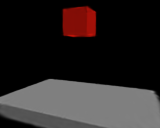
\includegraphics[width=.34\linewidth]{../../../output/npc-vision/4d4c8917622509ff51e06db391ab30b0c5af04dd86da6f865a96bfdb9482c96a/val-00.png}\hspace{5mm}
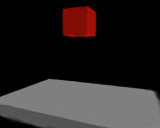
\includegraphics[width=.34\linewidth]{../../../output/npc-vision/4d4c8917622509ff51e06db391ab30b0c5af04dd86da6f865a96bfdb9482c96a/val-01.png}
\end{center}
这两张是重建结果。两个机位都没有参与训练，图中的箱子仍悬在烘焙时的位置。对两个机位分别与留出的原图比较，每个 RGB 分量先除以 255，再计算平方误差的平均值 $E$。按 $-10\log_{10} E$ 换算，分别为 31.64 和 31.86 dB。这个数衡量像素颜色的接近程度。箱子后来有没有落地，则需要在游戏运行时查证。

游戏调用 \code{AskNpcVision} 时给出场景名称和问题。视觉服务先根据机位的关键词选取至多两张图，再把图片、物体名称及编号交给视觉模型。示例中的名称与编号由关卡作者标注。服务只接受这几张图里列出的编号。候选列表用于缩小搜索范围，照片中不在列表里的物体需要先在资料中补上。

模型作答耗时可能跨越好几个物理步。游戏可以继续更新，等异步结果准备好，再在场景线程调用 \code{CanPickUp}。引擎按编号查找物体，检查“可拿取”组件，并从手的位置向物体发出一条长度有限的射线。如果中间已多了一面墙，射线会先碰到墙。如果箱子已被别人拿走，查实体时就会失败。这里返回的是此次查询的结果，游戏随后决定怎样改变物品栏或场景。

\clearpage
\subsection{照片中的区域与指向}

“指出地台右侧的灰色台面”问的是地台的一部分。场景里只有整座地台的编号，给右侧台面另建一个实体也无助于画面定位。关卡作者可以直接在照片上标出这块区域。下图的框保存在实验台的 \code{Physics-Workshop.views.json}，名称是“地台右侧的灰色台面”。

\begin{figure}[H]\centering
\begin{tikzpicture}[x=.37mm,y=-.37mm]
  \node[anchor=north west,inner sep=0] at (0,0)
    {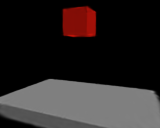
\includegraphics[width=59.2mm]{../../../output/npc-vision/4d4c8917622509ff51e06db391ab30b0c5af04dd86da6f865a96bfdb9482c96a/val-00.png}};
  \draw[yellow!85!white,line width=1.1pt] (108,96) rectangle (136,112);
  \fill[yellow!85!white] (122,104) circle[radius=1.2];
  \draw[blue,thick] (137,104) -- (173,104);
  \node[anchor=west,align=left,font=\small] at (175,104) {标注框中心 $(122,104)$\\左上角为 $(0,0)$};
\end{tikzpicture}
\caption{Brush 从重建的三维高斯渲染出机位 val-00，原图为 $160\times128$ 像素。黄色框与中心点按项目索引叠加。}
\end{figure}

照片中的一点只能确定一个观察方向。相机在世界坐标的 $(2.383,2.121,5.507)$，焦距折合 145 像素，光轴穿过图心 $(80,64)$。标注中心比图心向右 42 像素、向下 40 像素。在相机坐标里，向右为正 $x$，向上为正 $y$，镜头朝负 $z$。因此，从镜头出发，在正前方一个单位远的平面上，这个像素对应的位置是
\[
    \bigl((122-80)/145,\ (64-104)/145,\ -1\bigr).
\]
\code{bake\_npc\_views.py} 的 \code{region\_directions} 用拍摄时的相机旋转把这个向量转到世界坐标，再除以长度，得到 $(-0.106,-0.372,-0.922)$。在编辑器“NPC 观察”里按“从拍摄机位看向该处”，相机便回到照片的起点，沿这个方向观察。游戏中也可以把方向交给朝向或指示动作。换一个站位时须保留射线原来的起点，沿同一方向平移并不能保证指到原处。

测试利用场景中台面高度 $y=0$ 验算方向。照片射线与平面的交点约为 $(1.779,0,0.255)$，落在半宽 3 米、半深 2 米的台面内。交点只用于这间实验室的验证。普通单张照片没有给出目标距离，游戏取得的是从拍摄机位出发的世界射线。离线索引假定照片已经校正镜头畸变，机位和游戏采用同一套世界坐标。相机局部坐标与矩阵列的约定可对照 \href{https://docs.nerf.studio/quickstart/data_conventions.html}{Nerfstudio 的 Camera/view space 与 Camera extrinsics}。

\clearpage
\subsection{候选结果的读取与核验}

支持区域的游戏入口是 \code{AskNpcCandidate}。问“右边那个红箱子”仍然是在找箱子。服务选好图片，再把图中的实体和命中关键词的区域列在同一张表里。实验台里的箱子编号为 103，台面上的框在这次提问中暂用 104。模型选框时，服务把框内的实际像素裁出来再问一次。机位、框名、起点和方向都从已发图片的索引里取。模型自行报出的坐标、其他机位的引用和不存在的编号都会被丢弃。

游戏保留返回的 \code{future}，在后续更新中检查答案。下面是对应 \src{Redflag/src/Redflag/Scene/NpcVision.h}{NpcVision.h} 与 \src{RedflagForge/src/NpcVisionPanel.cpp}{NpcVisionPanel::Draw} 的调用节选；变量 \code{scene} 和 \code{camera} 是当前场景与编辑器相机。

\begin{lstlisting}[language=C++]
// (*@收到提问时保存 waiting，每次更新检查一次。@*)
if (waiting.valid() &&
    waiting.wait_for(std::chrono::seconds(0)) ==
    std::future_status::ready) {
    NpcVisionCandidate answer = waiting.get();
    if (answer.Region) {
        const NpcViewRegion& r = *answer.Region;
        camera.LookAt(r.Origin, r.Origin + r.Direction);
    } else if (answer.Entity) {
        bool reachable = CanPickUp(scene, *answer.Entity,
                                   hand, reachInMeters);
    }
}
\end{lstlisting}

调用 \code{get()} 会取走结果，后续更新通过 \code{valid()} 知道这次提问已经结束。正式面板还会检查提问时的场景是否仍然打开。只有持有实体编号并已启动物理模拟时，面板才调用拾取查询。两个字段都为空表示没有选出候选。C++ 游戏可以使用上述接口；目前分发的 C\# ScriptCore 只提供现有的实体变换和输入等脚本入口。

本机用 Qwen3-VL-2B 分别读了随仓图片和一次从头训练 800 步后导出的图片。在每组中用中文、英文各问一次，找台面时均选中右侧的框，找“右边的红箱子”时均选中实体 103。把两张图片第 65 行至底部涂黑，保留箱子和文字标签，模型在两种语言中均返回空。早期只让它选编号时，中文提问曾让模型在台面被遮掉后仍选中该处。裁图复查减少了这组样本里的误选。这里总共只有一处有标注的台面，同色材质、严重遮挡和换房间都需要另测。

\readings{\href{run:../npc-vision/regions.json}{逐项识图记录与图片校验值}\quad \href{https://repo-sam.inria.fr/fungraph/3d-gaussian-splatting/}{Kerbl 等，3D Gaussian Splatting，SIGGRAPH 2023}\quad
\href{https://github.com/ArthurBrussee/brush/releases/tag/v0.3.0}{Brush 0.3.0}\quad
\href{https://nvidia-omniverse.github.io/PhysX/physx/5.6.1/docs/SceneQueries.html}{PhysX 场景查询}}
